\PassOptionsToPackage{svgnames}{xcolor}
\documentclass[10pt]{beamer}
\usepackage{booktabs}
\usepackage{caption}
\usepackage{lmodern}
\usepackage{amsmath}
\usepackage{amssymb,amsmath}
\usepackage{ifxetex,ifluatex}
\usepackage{fixltx2e} % provides \textsubscript
\ifnum 0\ifxetex 1\fi\ifluatex 1\fi=0 % if pdftex
\usepackage[T1]{fontenc}
\usepackage[utf8]{inputenc}
\else % if luatex or xelatex
\ifxetex
\usepackage{mathspec}
\else
\usepackage{fontspec}
\fi
\defaultfontfeatures{Ligatures=TeX,Scale=MatchLowercase}
\fi
\providecommand{\tightlist}{%
\setlength{\itemsep}{0pt}\setlength{\parskip}{0pt}}
\setcounter{secnumdepth}{0}
\usepackage{xcolor}
\usepackage{graphicx}

% There are many different themes available for Beamer. A comprehensive
% list with examples is given here:
% http://deic.uab.es/~iblanes/beamer_gallery/index_by_theme.html
% You can uncomment the themes below if you would like to use a different
% one:
%\usetheme{AnnArbor}
%\usetheme{Antibes}
%\usetheme{Bergen}
%\usetheme{Berkeley}
%\usetheme{Berlin}
%\usetheme{Boadilla}
%\usetheme{boxes}
%\usetheme{CambridgeUS}
%\usetheme{Copenhagen}
%\usetheme{Darmstadt}
\usetheme{metropolis}
\setbeamertemplate{itemize subitem}[triangle] % Pour le deuxième niveau
\setbeamertemplate{itemize subsubitem}[square] % Pour le troisième niveau
%\setbeamerfont*{itemize item}{size=\scriptsize}
\setbeamercolor{itemize item}{}
\setbeamercolor{itemize subitem}{fg=orange}
\setbeamercolor{itemize subsubitem}{fg=orange}
\setbeamerfont{headline}{size=\Large}
%\usetheme{default}
%\usetheme{Frankfurt}
%\usetheme{Goettingen}
%\usetheme{Hannover}
%\usetheme{Ilmenau}
%\usetheme{JuanLesPins}
%\usetheme{Luebeck}
%\usetheme{Madrid}
%\usetheme{Malmoe}
%\usetheme{Marburg}
%\usetheme{Montpellier}
%\usetheme{PaloAlto}
%\usetheme{Pittsburgh}
%\usetheme{Rochester}
%\usetheme{Singapore}
%\usetheme{Szeged}
%\usetheme{Warsaw}


\title{Correlated bivariate Normal competing risks%  -- simulation findings in an ill-posed problem
}

% A subtitle is optional and this may be deleted
\subtitle{ -- simulation findings in an ill-posed problem}

\author{Malcolm~Hudson\inst{1,2} \and Valerie~Gares \inst{3} \and Maurizio~Manuguerra\inst{1} \and Val~Gebski\inst{2}}
% - Give the names in the same order as the appear in the paper.
% - Use the \inst{?} command only if the authors have different
%   affiliation.
%\institute[Macquarie University] % (optional, but mostly needed)
\institute
{
  \inst{1}%
  Macquarie University \hfill 
\includegraphics[width=1.75cm,height=1.75cm,keepaspectratio]{logo/MU_logo_h.pdf}
  \and
  \inst{2}%
  NHMRC Clinical Trials Centre \hfill 
\includegraphics[width=1.5cm,height=1.5cm,keepaspectratio]{logo/logoUSyd.pdf}\\
  University of Sydney
  \and
  \inst{3}%
  INSA Rennes
}

\date{ISCB ASC 2018, Melbourne}

\subject{Competing Risks for bivariate Normal}
% This is only inserted into the PDF information catalog. Can be left
% out. 

% If you have a file called "university-logo-filename.xxx", where xxx
% is a graphic format that can be processed by latex or pdflatex,
% resp., then you can add a logo as follows:
%\titlegraphic{    
%  
\includegraphics[width=2cm,height=2cm,keepaspectratio]{logo/MU_logo_h.pdf}~\hfill~%
%  
\includegraphics[width=1.5cm,height=1.5cm,keepaspectratio]{logo/logoUSyd.pdf}%
%}
% \pgfdeclareimage[height=0.5cm]{MU-logo}{MQlogo.png}
% \logo{\pgfuseimage{MU-logo}}
%\logo{%
%    
\includegraphics[width=2cm,height=2cm,keepaspectratio]{MU_logo_h.pdf}~%
%    
\includegraphics[width=1.5cm,height=1.5cm,keepaspectratio]{../../logoUSyd.pdf}%
%}
\newcommand{\nologo}{\setbeamertemplate{logo}{}}

% Let's get started
\begin{document}

\begin{frame}
  \titlepage
\end{frame}

\begin{frame}{Outline}
  \tableofcontents
  % You might wish to add the option [pausesections]
\end{frame}

 \begin{frame}
  \frametitle{Competitive risks}
  \framesubtitle{Example}
\small\begin{itemize}
 \item Study time to  several events in competition (24 patients): 

   \begin{itemize}
  \item Myocardial infarction (MI) %  or  Cardiovascular death (CVD)
 $\rule[0.3ex]{1cm}{.3pt}\times$ (10)
\item Death from other causes
  ${\color{gray}{\rule[0.3ex]{1cm}{.5pt}\times}} $ (8)
\item Censoring
 $\cdots \circ $ (6)
  \end{itemize}
 \begin{center}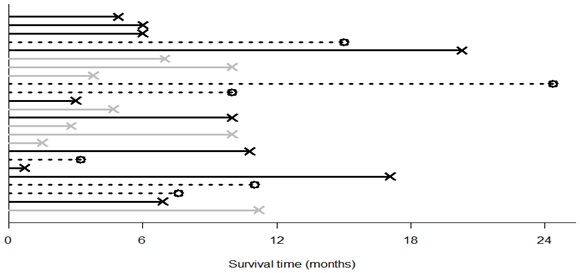
\includegraphics[height=3cm]{censure.jpg}\end{center}

  \item {\color{DarkBlue}{Patient status:}}\\
  
  \begin{tabular}{p{4cm}ll}
 Myocardial infarction 
 &\visible<2->{{\color{DarkBlue}{$\Rightarrow$}}}&\visible<2->{{\color{orange}{Event of interest  }}}\\
%Cardiovascular death
%  &\visible<2->{{\color{DarkBlue}{$\Rightarrow$}}}&\visible<2->{{\color{orange}{Event of interest  }}}\\
     Withdraw from study
   &\visible<2->{{\color{DarkBlue}{$\Rightarrow$}}}&\visible<2->{{\color{orange}{Censoring }}}\\
    Death from other causes
&\visible<2->{{\color{DarkBlue}{$\Rightarrow$}}}&\only<2>{{\color{orange}{Censoring} }}\only<3->{{\color{red}{\textbf{Competing event}}}}  \\
\end{tabular}

\item[] \visible<2>{{\color{red}{Introduces dependence between censoring and event}}}
\item[] \visible<3>{{\color{red}{Respects independent censoring assumption in SVA}}}
  \end{itemize}

\end{frame}



  
 
%{\nologo

% Section and subsections will appear in the presentation overview
% and table of contents.
\section{Bivariate Normal Censored Linear Model}

\begin{frame}{Correlated competing risks model}
  \begin{itemize}
  \item
    {\color{DarkBlue}{Bivariate Normal Censored Linear Model}} (bnc lm)
    \begin{itemize}
    \item
      Log-Time to {\color{DarkBlue}{\emph{first occurring}}} event
    \item
      Two events: $Y \sim \mbox{BVN}(\mu,\Sigma) $
    \item
      lm: $\mu = X B$ with $B=\left[ \beta_{ik} \right]$
    \item
      \emph{bnc} lm for observed data: \color{red}{$y=\min (Y_1, Y_2, C)$} and  \color{red}{$D=1,2,0$}
    \item Observations $(y,D)$ comprise \emph{first-event data} 
    \end{itemize}
  \item
    {\color{DarkBlue}{Estimation}}
    \begin{itemize}
    \item ML solution 
    \item
      ML $\leftarrow$  MPL
    \item
      EM algorithm uses imputed times to non-occurring event
    \end{itemize}
  \item 
   {\color{DarkBlue}{Imputation}}
    \begin{itemize}
    \item Conditional moments
      \( \mathbb{E} (Y_1| Y_1 > y, Y_2=y, \, D=2) \)
    \item
      \( \mathbb{E} (Y_1| Y_1 > y, Y_2 > y, \, D=0) \)
    \item 
    \( \mathbb{E} (Y_1^2| Y_1> y, Y_2=y,\, D=2) \) 
    \item
    \ldots \emph{etc}
    \end{itemize}
  \end{itemize}
\end{frame}




\section{Simulation Aim, Methods}

\begin{frame}{Simulation Goals}
\begin{itemize}
\item
  {\color{DarkBlue}{Aim:}} parametric estimation of \alert{first-event data} from correlated
  BVN competing risks

  \begin{itemize}
  \item
    Sampling distribution (\alert{bias, variance}) of MPL estimation of
    BVN parameters in one- and two- sample datasets of first-event times
  \item
    Sampling distribution of mean difference estimated between Treated
    and Control subjects
  \end{itemize}
\end{itemize}
\end{frame}
% -----------------------------------------------------------------------

\hypertarget{results}{%
\section{Simulations}\label{simulations}}

\begin{frame}[fragile]{Methods}
\protect\hypertarget{methods}{}

\begin{itemize}
\tightlist
\item
  One- and two-sample simulations, BVN and \emph{non-}Normal copula
  (with Normal margins)

  \begin{itemize}
  \tightlist
  \item
    Parameters varying

    \begin{enumerate}
    [i.]
    \tightlist
    \item
      Sample size (100, {\color{red}{400}}, 1000)  {\color{red}{why not 500}}
    \item
      Mean difference event-of-interest to competing-event (0, 0.5, 1)
    \item
      Event probability (complement \emph{censoring fraction}) $\to$ prob event-of-interest occurs before \texttt{eof}
        \begin{itemize}
        \tightlist
        \item[~~-]
          Surviving fractions (1, 0.8, 0.6)
        \item[~~-]
          Competing event censoring \emph{not} included
        \end{itemize}
    \item
      \alert{Correlation} \(\rho \in (-0.5,-0.25, 0, 0.25, 0.5)\)
    \item
      \alert{Treatment benefit} (mean difference between \emph{Treated
      and Controls, 2 sample only})
    \end{enumerate} % params varying
  \end{itemize}

\item
  Parallel simulation computation
  \begin{itemize}
  \tightlist
  \item
    \textbf{simsalapar} R package Hofert and Mächler (2016)
  \end{itemize}

\item
  Fixed-point accelerated EM iterations Bobb and Varadhan (2014)
\item
  estimation conducted in our R package \textbf{bnc}
\end{itemize}

\end{frame}

\setbeamertemplate{itemize subitem}[triangle] % Pour le deuxième niveau
\setbeamertemplate{itemize subsubitem}[square] % Pour le troisième niveau
%\setbeamerfont*{itemize item}{size=\scriptsize}
\setbeamercolor{itemize item}{}
\setbeamercolor{itemize subitem}{fg=orange}
\setbeamercolor{itemize subsubitem}{fg=orange}

\setbeamerfont{headline}{size=\Large}\section{Results:}

%%

\section{{1-sample} estimation of correlation}
\protect\hypertarget{estimation-of-rho-one-sample}{}


\begin{frame}{squareEM iterations (n=1000)}

\begin{table}[htbp]
  \centering\scriptsize
  \begin{tabular}{*{2}{l}*{3}{r}}
    \toprule
    cs & \( \rho \) \textbar\ beta2 & \multicolumn{1}{c}{0} & \multicolumn{1}{c}{0.5} & \multicolumn{1}{c}{1} \\
    \midrule
    1 & -0.5 & 36 & 95 & 93 \\
    & -0.25 & 83 & 107 & 154 \\
    & 0 & 107 & 142 & {\color{red}250} \\
    & 0.25 & 90 & 127 & {\color{red}250} \\
    & 0.5 & 112 & 227 & {\color{red}250} \\ \addlinespace[3pt]
    0.8 & -0.5 & 36 & 90 & 116 \\
    & -0.25 & 88 & 108 & 243 \\
    & 0 & 119 & 163 & {\color{red}250} \\
    & 0.25 & 146 & 219 & {\color{red}250} \\
    & 0.5 & 141 & 248 & {\color{red}250} \\ \addlinespace[3pt]
    0.6 & -0.5 & 78 & 105 & {\color{red}250} \\
    & -0.25 & 117 & {\color{red}250} & 235 \\
    & 0 & 134 & 212 & {\color{red}250} \\
    & 0.25 & 159 & 240 & {\color{red}250} \\
    & 0.5 & 184 & {\color{red}250} & {\color{red}250} \\
    \bottomrule
  \end{tabular}
  \caption*{max number iterations to converge, nsim=100}
  \label{tab:ft1b}
\end{table}
\end{frame}




\begin{frame}{Correlation (n=100)}

\begin{center}
  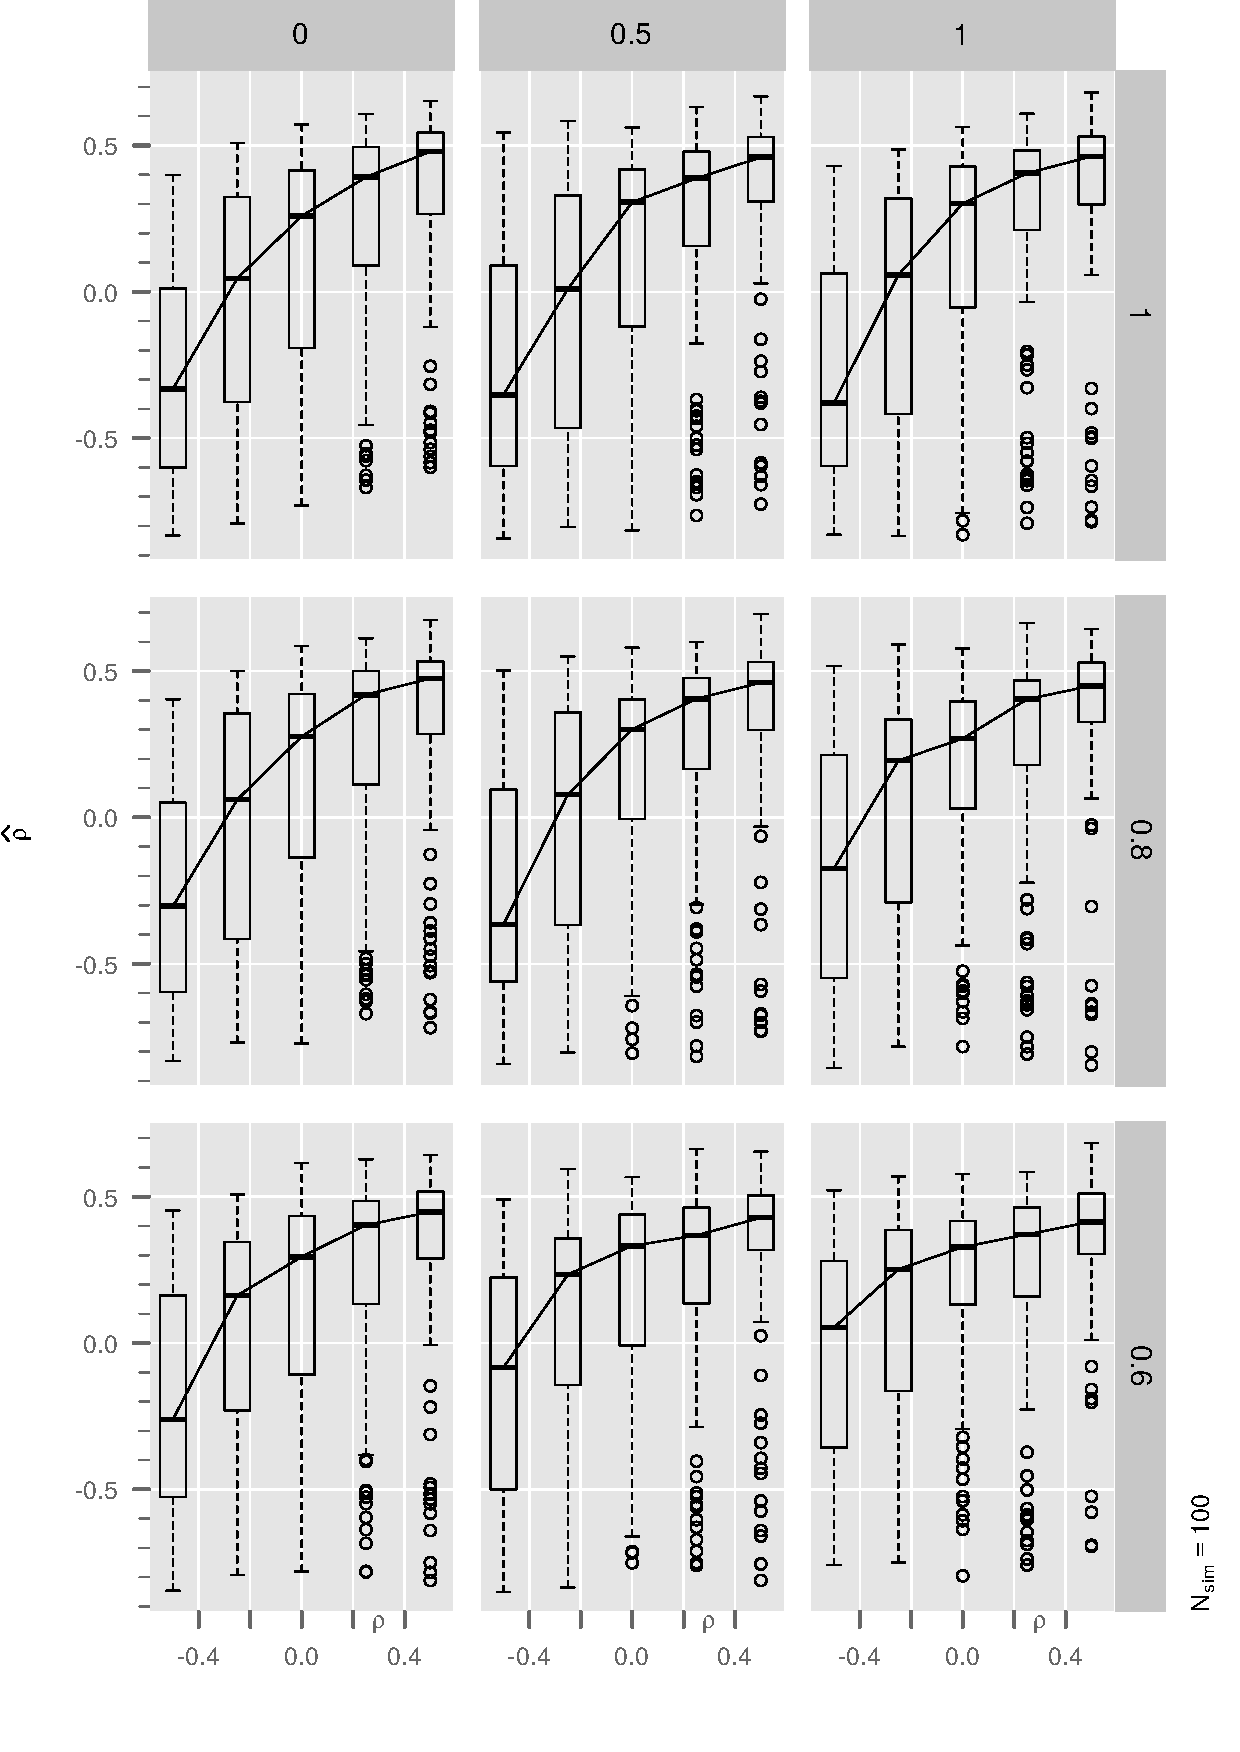
\includegraphics[trim= 0cm 0cm 0cm 11.75cm, clip, scale=0.475]{Figure1/tbl1_n100_rho_mayplot.pdf}
\end{center}

\end{frame}

\begin{frame}{Correlation, n=500 (Density plot)}

\begin{center}
  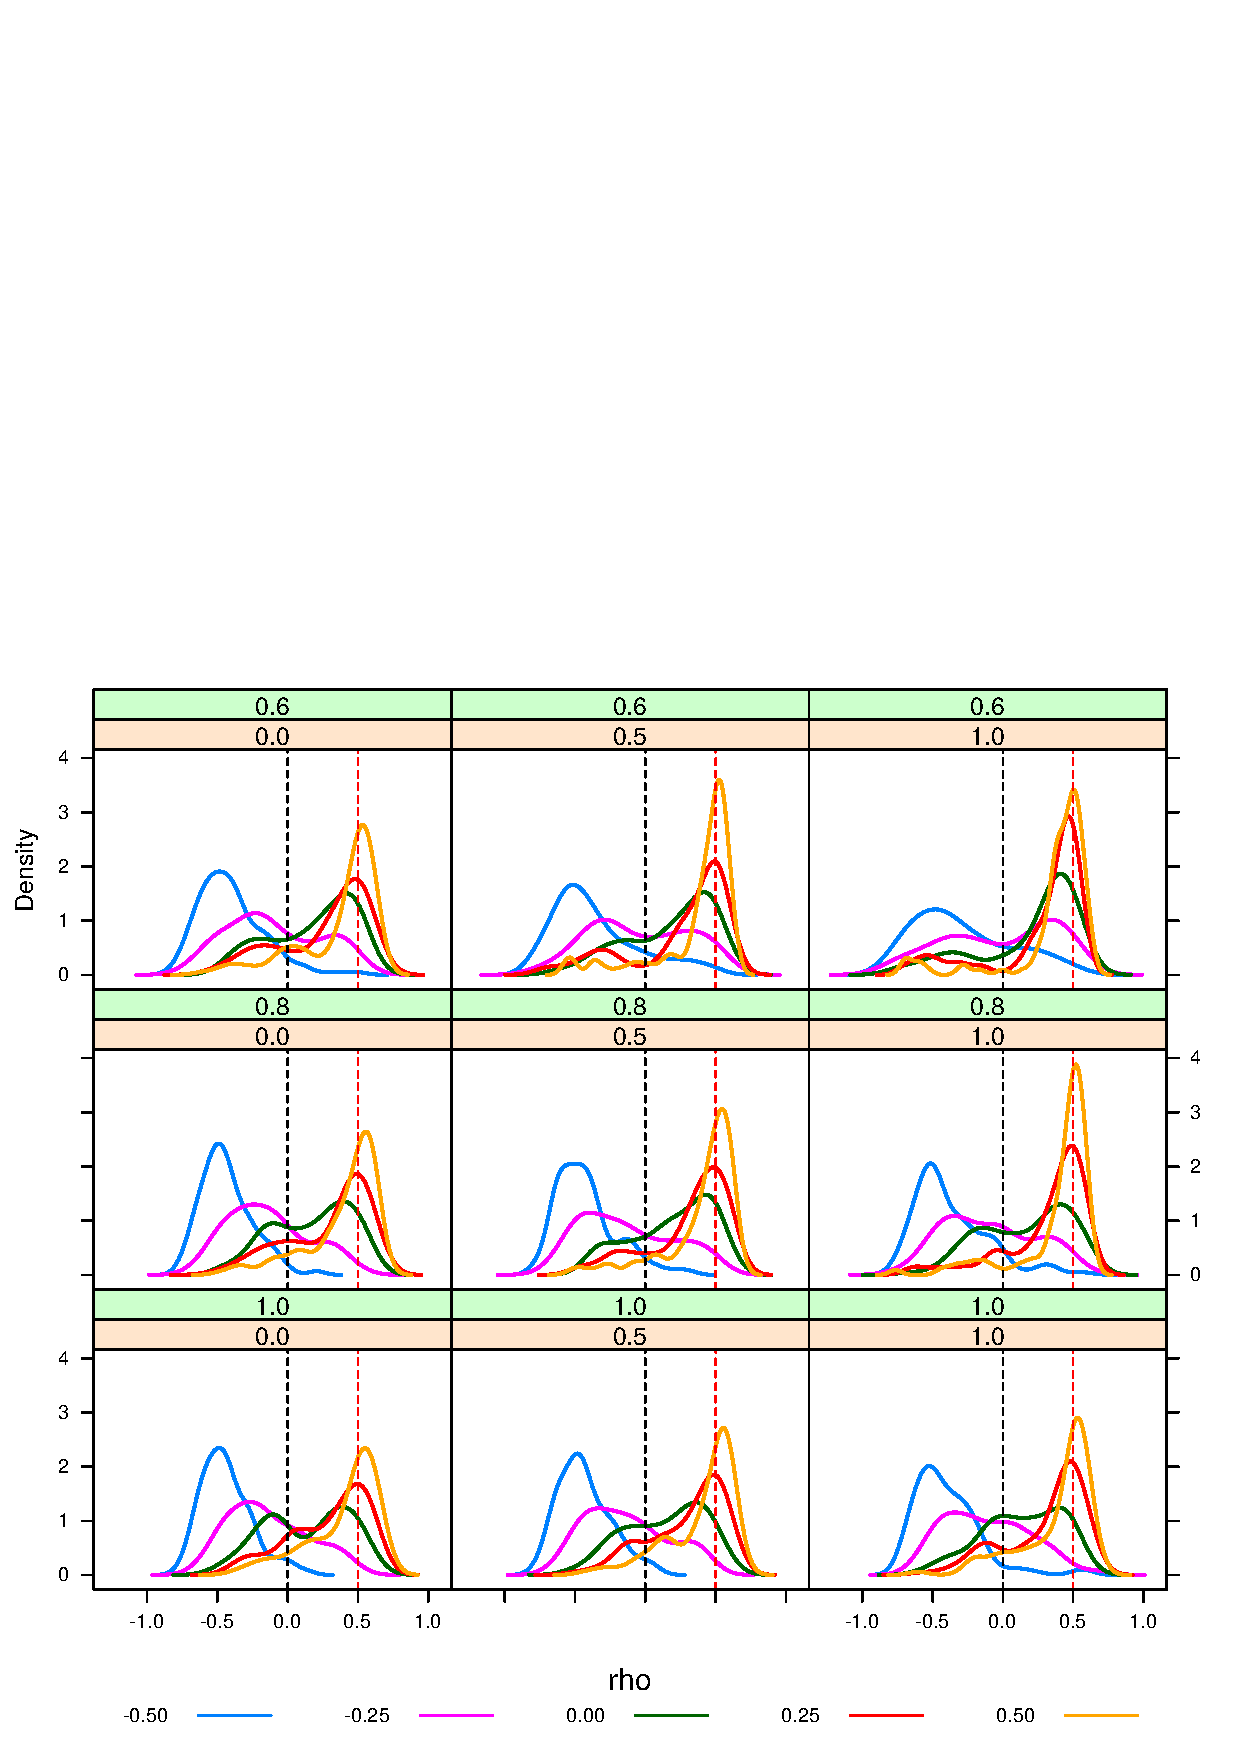
\includegraphics[trim= 0cm 0cm 0cm 11.75cm, clip, scale=0.47]{Figure1/tbl1densityPlot_n500.pdf} % width=1.00\textwidth, clip,, [scale=0.67]
\end{center}

\end{frame}

% ==============================================================================================
\section{{2-sample} estimation of treatment benefit}
\protect\hypertarget{two-samples}{}

\begin{frame}{Treatment Benefit $\hat{\Delta}=\hat{\beta}_{21}$ (n=1000)} % 3b: n=1000
\begin{table}[htbp]
  \centering\scriptsize
  \begin{tabular}{*{2}{l}*{4}{r}}
    \toprule
     & beta12 & \multicolumn{2}{c}{0} & \multicolumn{2}{c}{1} \\
    \cmidrule(lr){3-4} \cmidrule(lr){5-6}
    cs & \( \rho \) \textbar\ deltaTreat & \multicolumn{1}{c}{0} & \multicolumn{1}{c}{0.5} & \multicolumn{1}{c}{0} & \multicolumn{1}{c}{0.5} \\
    \midrule
    1 & -0.5 & -0.00 & 0.50 & 0.00 & 0.51 \\
    & -0.25 & -0.00 & 0.48 & -0.01 & 0.50 \\
    & 0 & 0.00 & 0.46 & 0.00 & 0.50 \\
    & 0.25 & -0.01 & 0.49 & 0.00 & 0.49 \\
    & 0.5 & -0.00 & 0.52 & -0.00 & 0.49 \\ \addlinespace[3pt]
    0.8 & -0.5 & -0.00 & 0.50 & 0.00 & 0.50 \\
    & -0.25 & -0.00 & 0.48 & 0.01 & 0.49 \\
    & 0 & 0.01 & 0.49 & 0.00 & 0.49 \\
    & 0.25 & -0.00 & 0.48 & -0.01 & 0.48 \\
    & 0.5 & -0.01 & 0.51 & 0.01 & 0.51 \\ \addlinespace[3pt]
    0.6 & -0.5 & 0.02 & 0.49 & -0.01 & 0.48 \\
    & -0.25 & -0.02 & 0.52 & -0.00 & 0.48 \\
    & 0 & -0.01 & 0.49 & 0.01 & 0.48 \\
    & 0.25 & 0.02 & 0.49 & 0.01 & 0.50 \\
    & 0.5 & 0.00 & 0.51 & -0.01 & 0.51 \\
    \bottomrule
    \multicolumn{5}{l}{\footnotesize{medians of 100 replicates}} % \multicolumn{4}{l}{\textsuperscript{*}\footnotesize{The footnote}}
  \end{tabular}
%  \caption{b21 TreatDiff estimate: Table 3b, n=1000}
  \label{tab:ft21}
\end{table}

\end{frame}


%\begin{frame}{2-sample: Treatment Benefit, n=1000 (estimates)} % sf x beta12

%\begin{center}
%  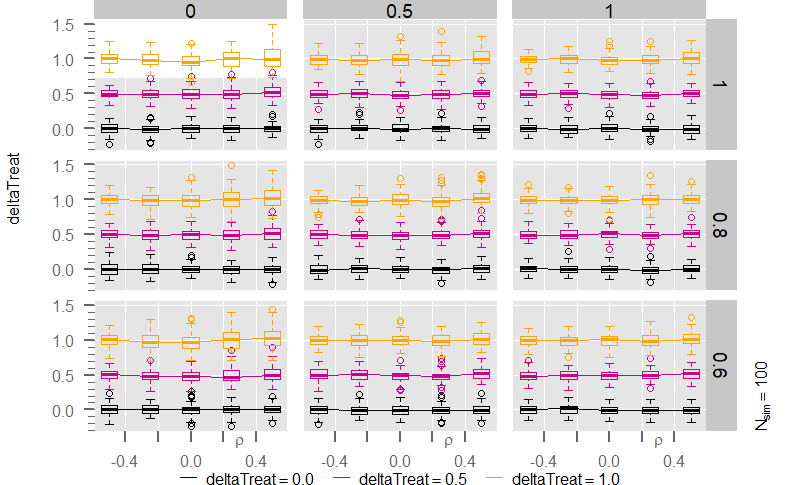
\includegraphics[width=1.00\textwidth]{Figure3/mayplot3-deltaTreat-n1000.png}
%\end{center}

%\end{frame}

%{Treatment Benefit, n=1000, sf=0.6 (density plots)}
%  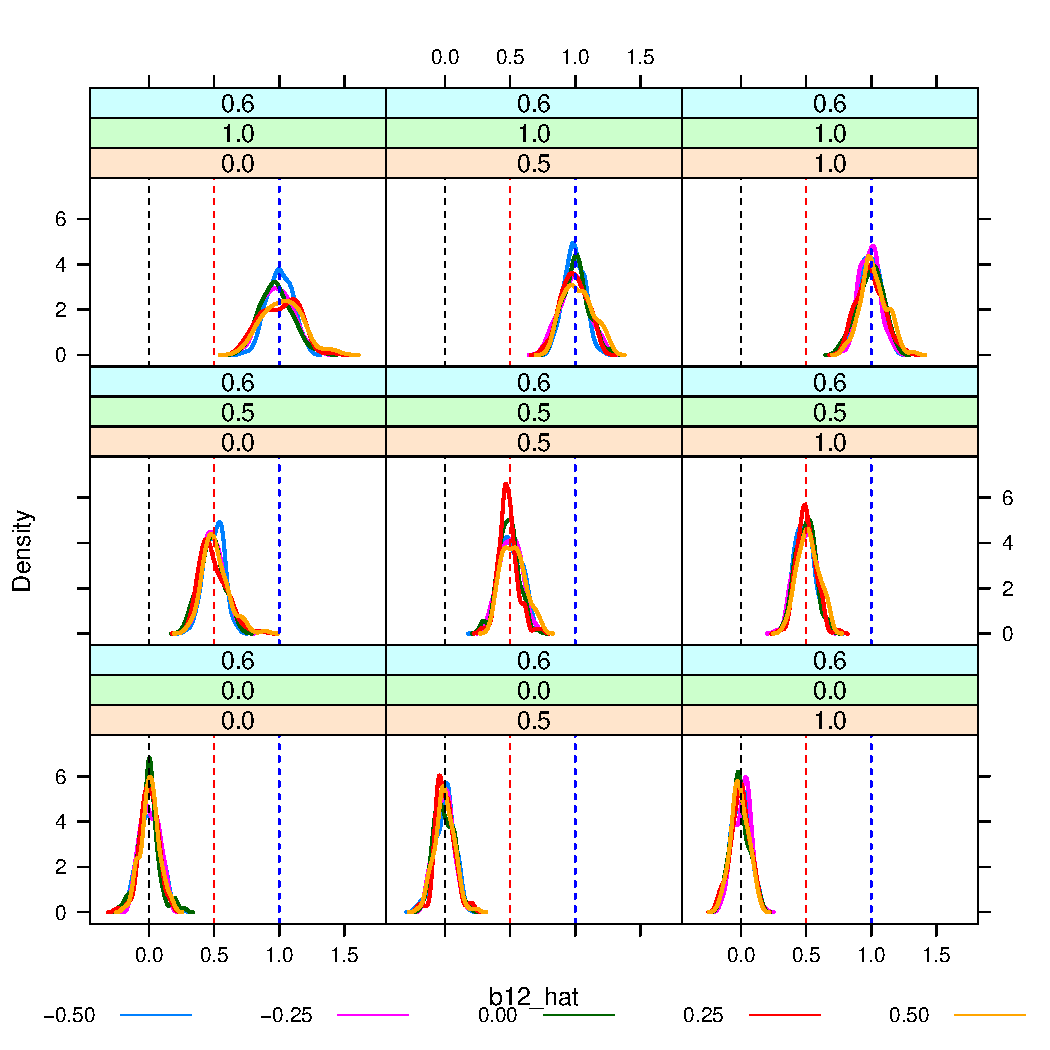
\includegraphics[scale=0.45]{Figure3/tbl3DensityPlots_n1000_003.pdf} % sf=0.6

\begin{frame}{Treatment Benefit, n=100 (estimates)} % sf x beta12

\begin{center}
  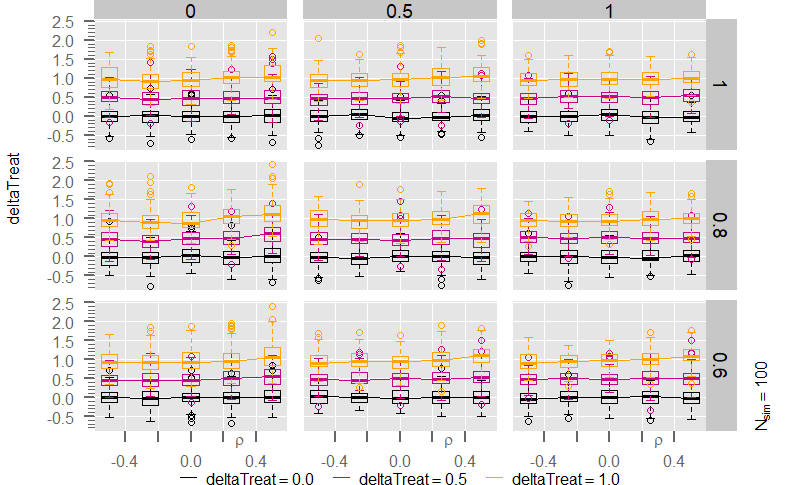
\includegraphics[width=1.00\textwidth]{Figure3/mayplot3-deltaTreat-n100.png}
\end{center}

\end{frame}

%  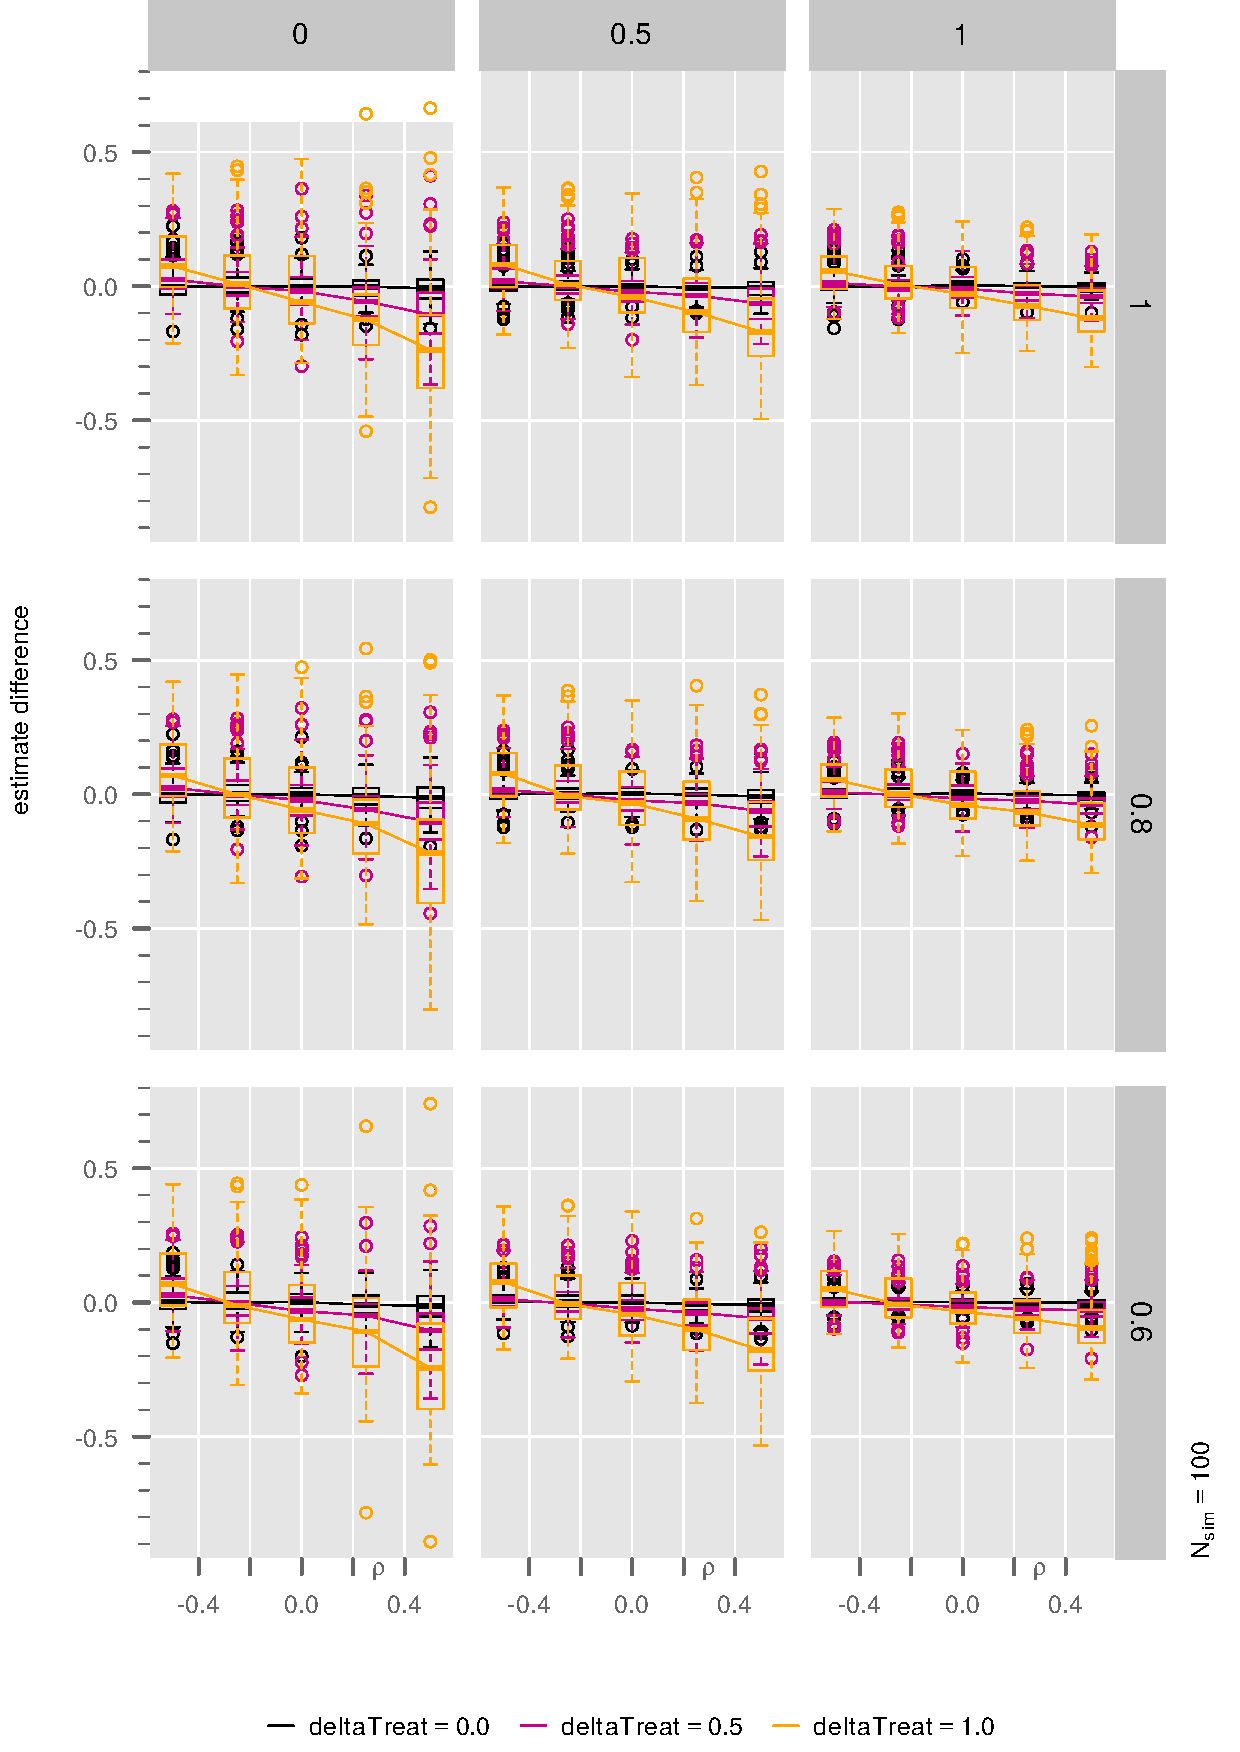
\includegraphics[width=0.95\textwidth]{Figure3/estimateDifferences2v12.pdf}


%\begin{frame}{2-sample: Treatment difference: BNC estimate  vs survreg coef ($\rho=0$)}

%\begin{center}
%  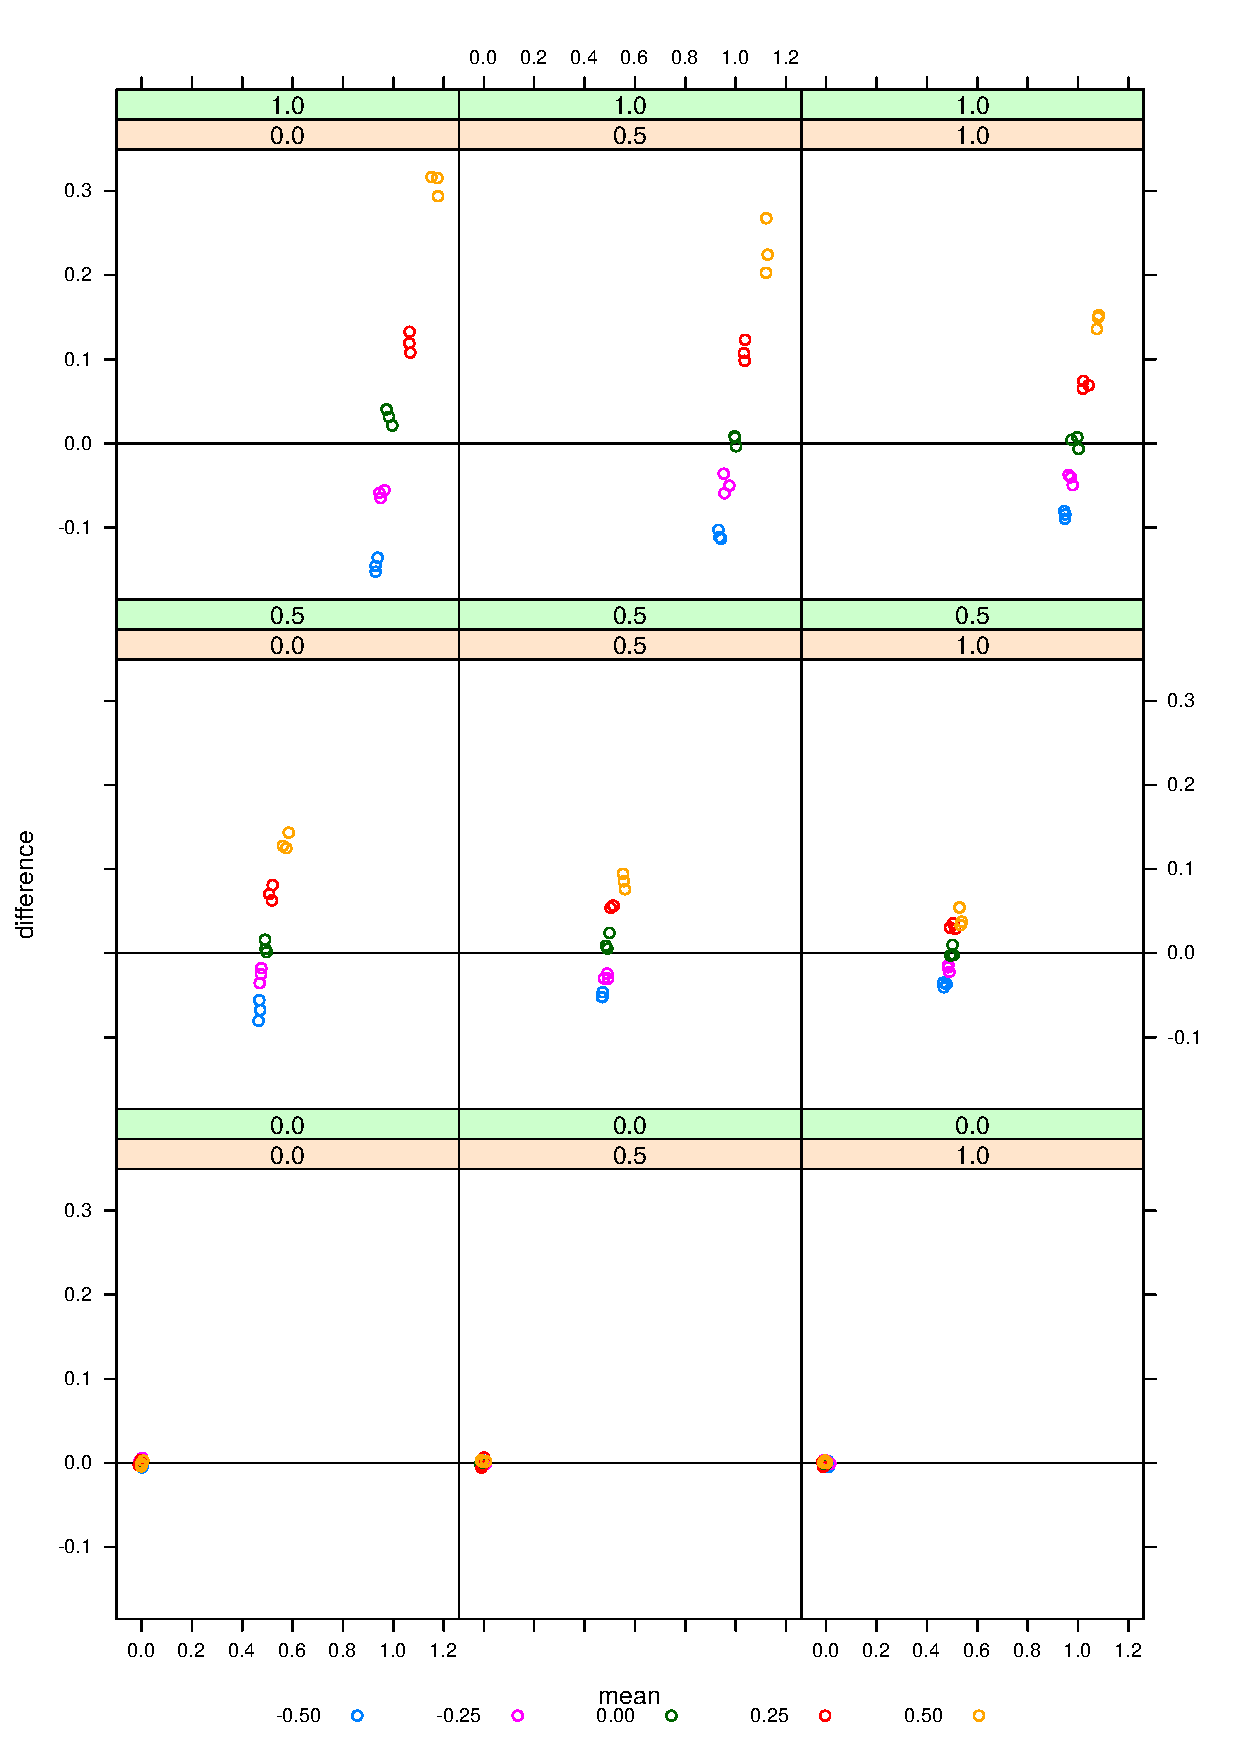
\includegraphics[height=0.95\textheight,width=0.95\textwidth]{%
%  Figure3/estimateDifferences2vs12v2.pdf%
%  }
%\end{center}

%\end{frame}


\begin{frame}{Treatment Benefit, n=1000, sf=0.6 (density plots)}

\begin{center}
  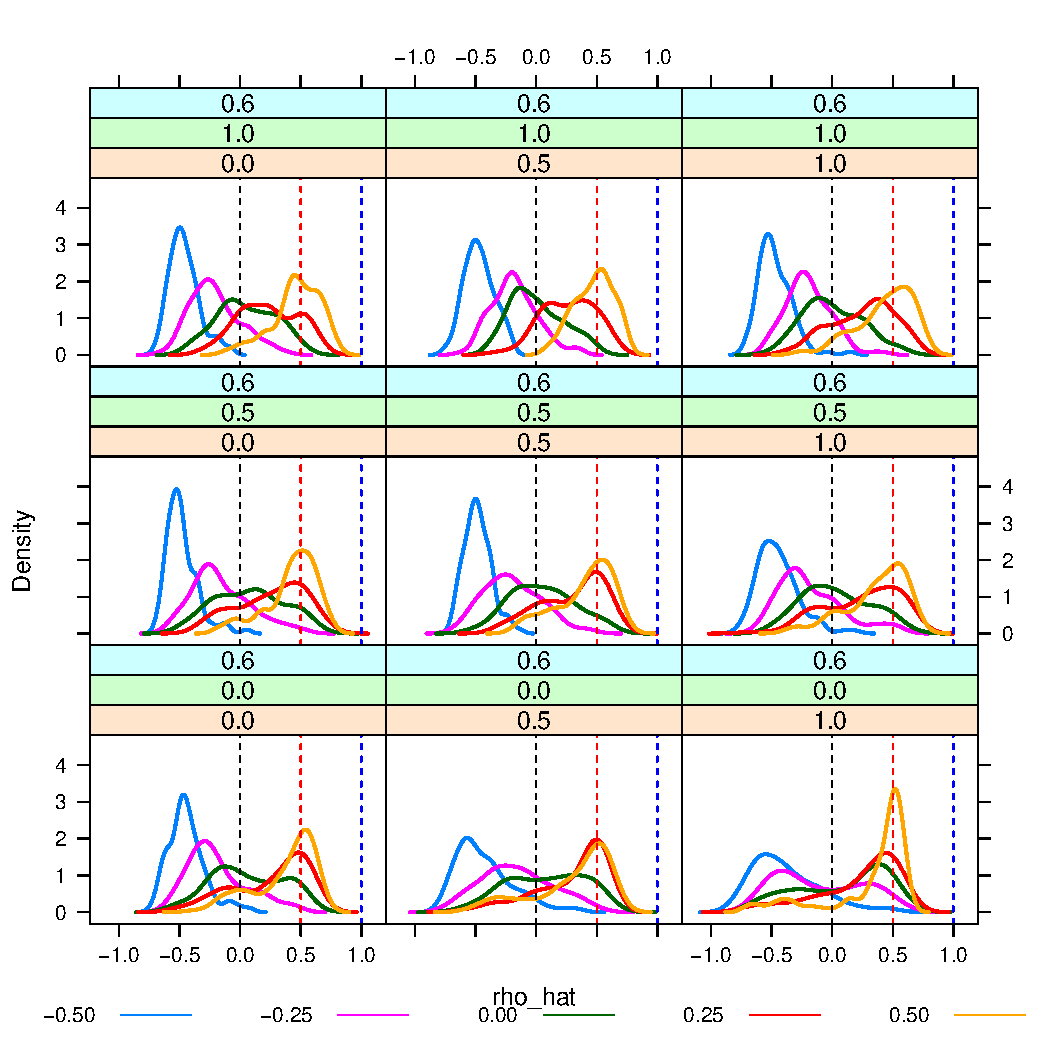
\includegraphics[scale=0.45]{Figure3/tbl3DensityPlots_rho_n1000_003.pdf} % sf=0.6
\end{center}

\end{frame}




% -------------------------------------------------------------------------

% \hypertarget{options}{%
% \section{Options}\label{options}}

\section{Follow-up}


\begin{frame}[fragile]{Fixed correlation, a la GEE}
\protect\hypertarget{fixed-correlation-a-la-gee}{}

\begin{itemize}
\tightlist
\item
  MPL solution with rho fixed
  \begin{itemize}
      \item \textit{Anderson and Olkin (1985)} (R package **bnc**)
  \end{itemize}
\end{itemize}




\begin{block}{Fixed correlation, rationale}

\begin{itemize}
\tightlist
\item
  Estimating \(\rho\) is unstable \(\ \Rightarrow\) fix its value a priori (to 0).
\item
  \(\rho=0\) is convenient

  \begin{itemize}
  \tightlist
  \item
    Competing event \(\to\) (further) independent censoring
  \item
    Fit regression coefficients of event 1 in
    \texttt{survival::survreg}
  \item
    Generalized Estimating Equations (GEEs)

    \begin{itemize}
    \tightlist
    \item
      Consistency/ unbiasedness to estimating regression coefficients?
    \item
      Likelihood scores with assumed covariance structure
    \end{itemize}
  \end{itemize}
\end{itemize}
\end{block}

\end{frame}

\begin{frame}{survreg coef of treatment benefit assuming $\rho=0$, n=100}

\begin{center}
  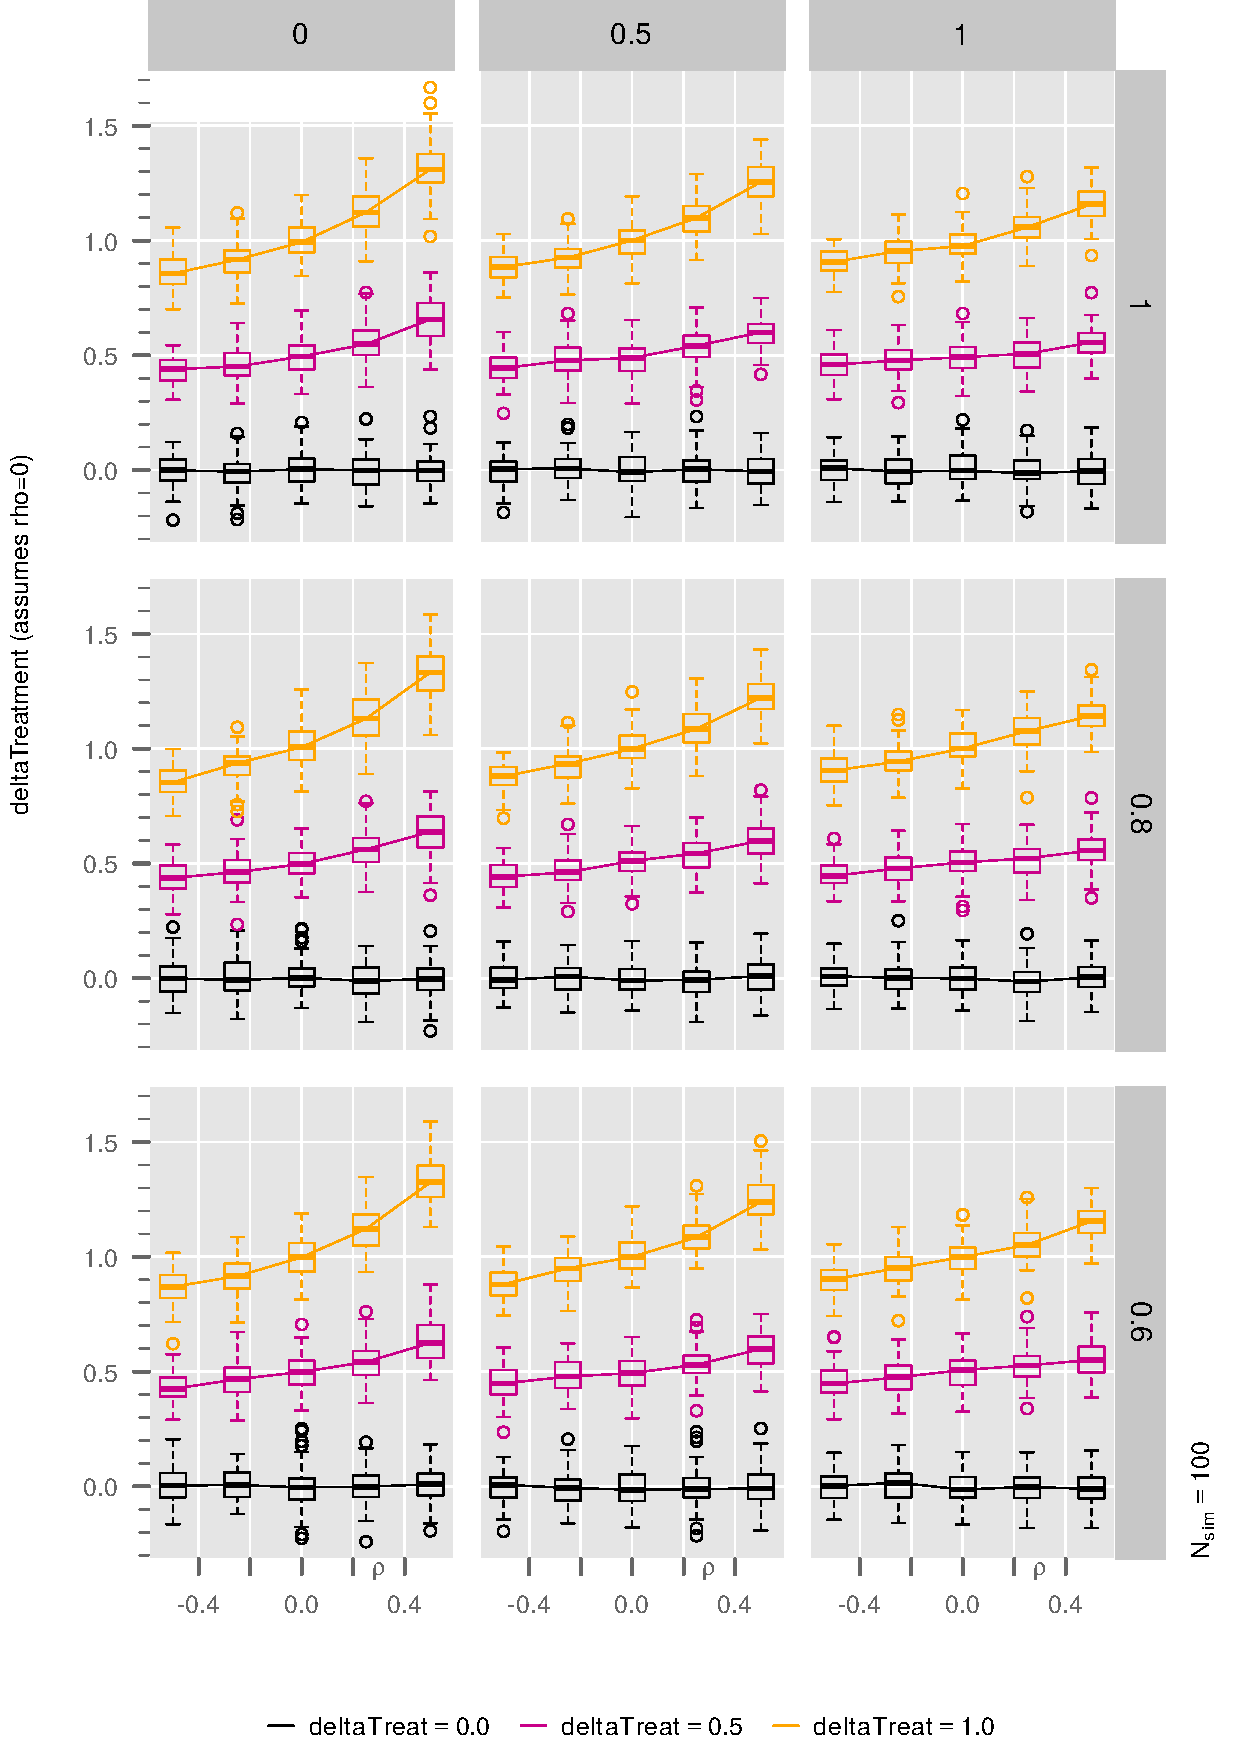
\includegraphics[width=1.00\textwidth]{Figure3/mayplot-coefTreat-n100-v2.pdf} % sf=0.6 scale=0.45
\end{center}

\end{frame}


% -------------------------------------------------------------------------
\hypertarget{robustness-to-non-normality}{%
\section{Robustness to non-Normality}\label{robustness-to-non-normality}}

\begin{frame}{Frank copula}
\protect\hypertarget{frank-copula}{}

\begin{itemize}
\tightlist
\item
  We set standard Normal \emph{marginals}
\item
  Association parameter, Frank \(\theta\)

  \begin{itemize}
  \tightlist
  \item
    \(\theta \rightarrow \tau \rightarrow \rho\)
  \end{itemize}
\item
  \emph{Joint} distribution is \alert{non-} BVN
\end{itemize}

Simulate two-sample \alert{estimate of treatment benefit} with copula generated data. Shown below:
\begin{itemize}
  \tightlist
  \item n=100
  \item 100 simulations per cell ($\beta_{12}$ and sf (1.0, 0.8) versus $\theta$)
  \item $\beta_{12} \in 0$ (black), $0.5$ (purple), $1$ (orange)
  \item $\theta \in (-3.3057723, -1.4789574,    0, 1.4789574, 3.3057723)$
\end{itemize}
\end{frame}

\begin{frame}[fragile]{Treatment benefit (n=100)}

\begin{center}
  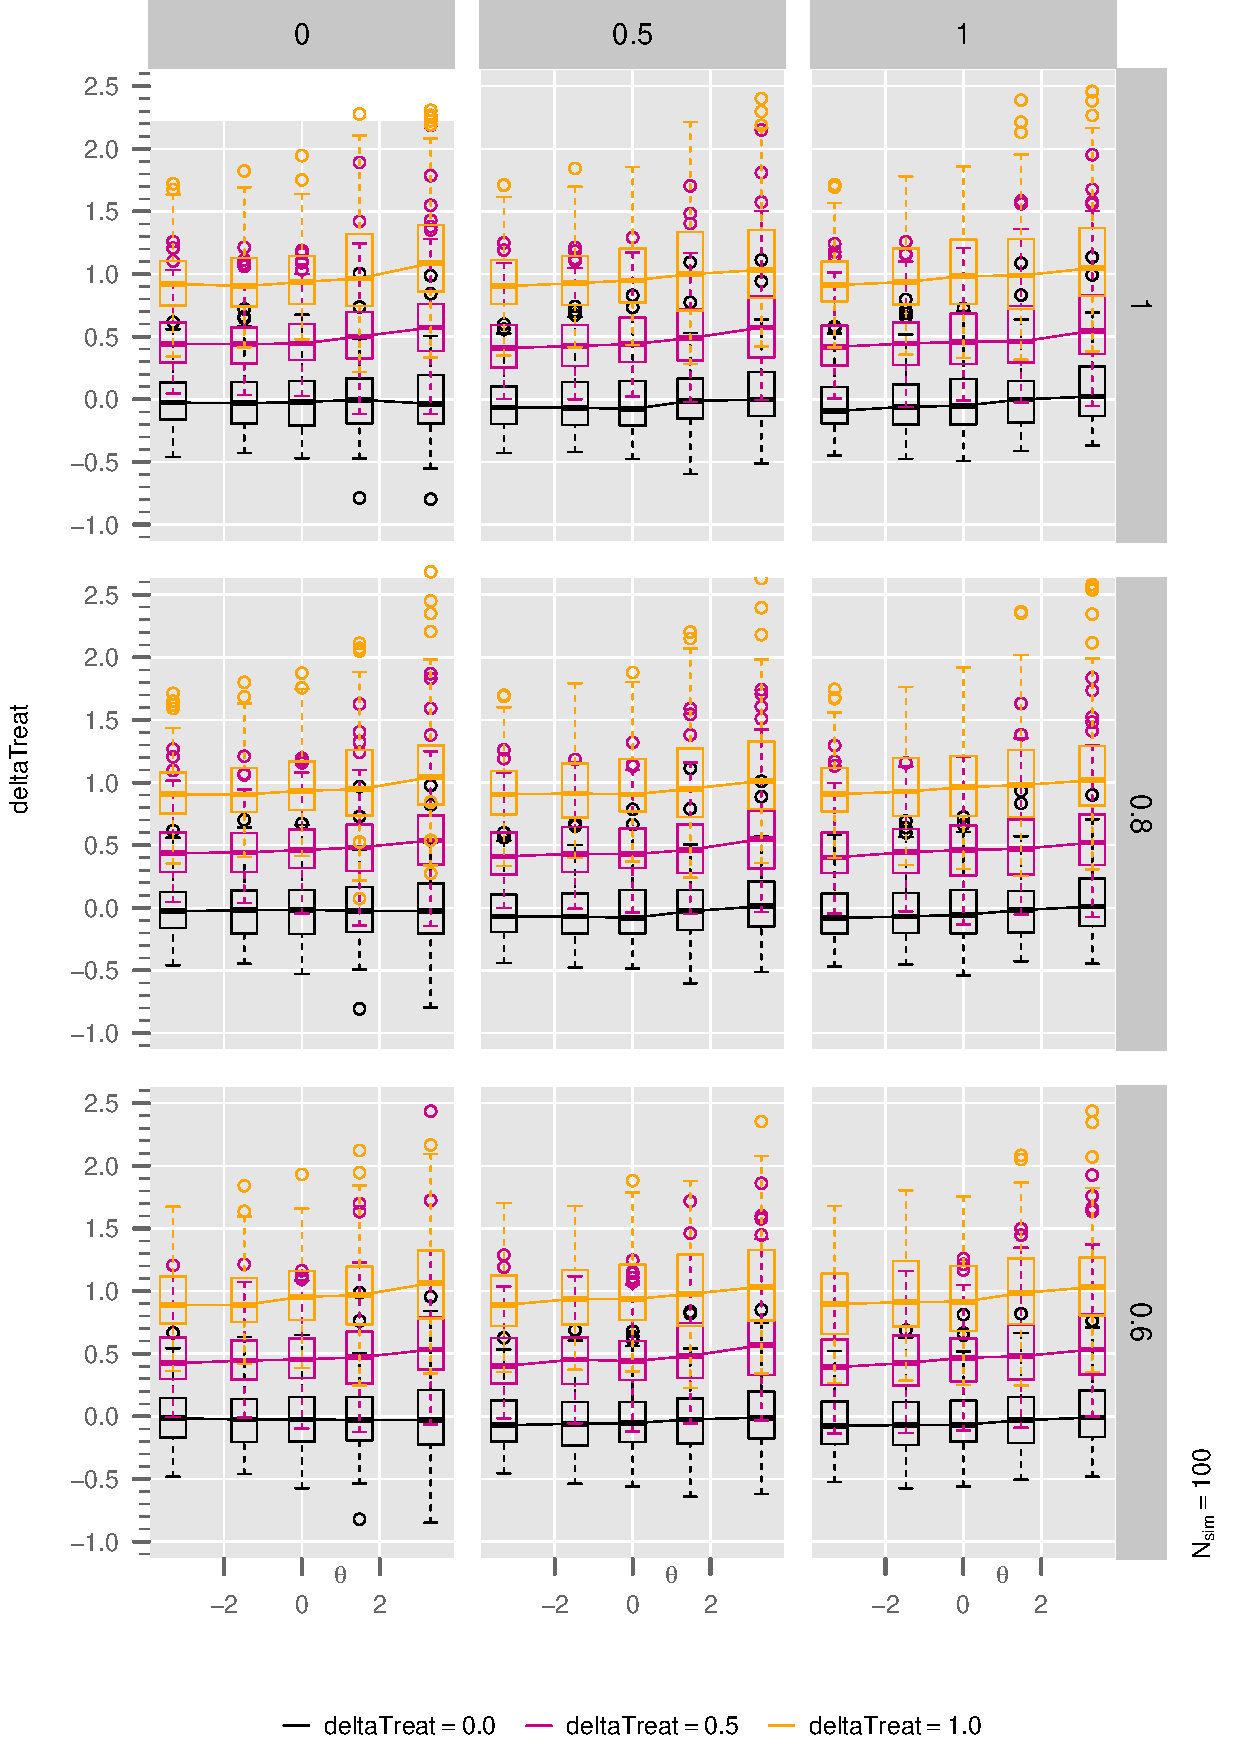
\includegraphics[width=0.95\textwidth]{Figure4/mayplot_deltaTreat.pdf}
\end{center}

\end{frame}


% Placing a * after \section means it will not show in the
% outline or table of contents.
\section*{Summing up}

\begin{frame}[fragile]{So you want to fit BVN to two competing risks?}
\protect\hypertarget{so-you-want-to-fit-bvn-to-two-competing-risks}{}
\setbeamercovered{transparent}
\begin{itemize}
\tightlist
\item<1->
  Optimize (e.g. \textemph{optim}) to maximize Likelihood function
  \item<2-> EM algorithm (\emph{safety first}) 
  \item<3-> Mildly
Penalize Likelihood, adjust EM alg for MPL
  \item<4-> Accelerate EM (Aitken via squareEM)
  \item<5-> Change start-point: initial small number of
EM iterations 
  \item<6-> R-package \textbf{bnc}
\end{itemize}

\only<1-4>{\alert{\emph{What could possibly go wrong?}}}
\begin{itemize}
\item<1> Singular Hessian, failure to remain in $-1 < \rho < 1$, method fails 
\item<2>
  \begin{enumerate}
  \item[i.] Be prepared to wait (forever) for convergence;
  \item[ii.] Convergence failure possible when $\hat{\rho}_{\mbox{ML}} = +1$ or $-1$
  \end{enumerate}
\item<3> Still very slow, but sure, convergence
\item<4> Very fast, but can fail to converge
\end{itemize}
\end{frame}


\begin{frame}{Conclusion}
  \begin{itemize}
  \item
    We fit a \alert{BVN censored model} for competing risks using a novel EM algorithm 
    (package \textbf{bnc}).
  \item
    Despite the \alert{ill-posed} model, estimation is feasible.\\
    {\color{DarkBlue}{Estimates:}} \\
   
    \begin{tabular}{ c l l }
    \hline
    $\rho$: &  \alert{correlation estimates} & highly variable ($n=1000)$ \\
    $\beta$: & \alert{regression coefficients}  &  precise (even for $n=100)$ \\ \hline  
    \end{tabular}
    
  \item Regression coefficients provide estimates of \alert{treatment benefit} 
  in a parametric \alert{AFT competing risks} survival model.
  \end{itemize}
  
  \begin{itemize}
  \item
    {\color{DarkBlue}{Outlook}}
    \begin{itemize}
    \item
      Need further comparison of estimates of $B$ fixing $\rho$ (e.g. assuming $\rho=0$) with MPL estimates of the BNC model.
    \item
      Asymptotic properties of this GEE-like procedure warrant investigation.
    \end{itemize}
  \end{itemize}
\end{frame}






% \hypertarget{references}{%

\section*{References}\label{references}

\begin{frame}[allowframebreaks]{References}
\label{References}

Aitkin, M. 1981. ``A Note on the Regression Analysis of Censored Data.''
\emph{Technometrics} 23 (2). American Statistical Association; American
Society for Quality: 161--63. \url{http://www.jstor.org/stable/1268032}.

Anderson, T.W. and Olkin, I. 1985. ``Maximum-likelihood estimation of the parameters of a multivariate normal distribution.''
\emph{Linear Algebra and its Applications} 70.  147--71. \url{https://doi.org/10.1016/0024-3795(85)90049-7}.

%\leavevmode\hypertarget{ref-Rpackage-turboEM}{}%
Bobb, J. F. and Varadhan, R. 2014. \emph{TurboEM: A Suite of
Convergence Acceleration Schemes for EM, MM and Other Fixed-Point
Algorithms}. \url{https://CRAN.R-project.org/package=turboEM}.

%\leavevmode\hypertarget{ref-Crowder1991}{}%
Crowder, M. 1991. ``On the Identifiability Crisis in Competing Risks
Analysis.'' \emph{Scandinavian Journal of Statistics}
18 (3): 223--33. \url{https://doi.org/10.2307/4616205}.

%\leavevmode\hypertarget{ref-Rpackage-simsalapar}{}%
Hofert, M. and  Mächler, M. 2016. ``Parallel and Other
Simulations in R Made Easy: An End-to-End Study.'' \emph{Journal of
Statistical Software} 69 (4): 1--44.
\url{https://doi.org/10.18637/jss.v069.i04}.

%\leavevmode\hypertarget{ref-JeongFine2007}{}%
Jeong, J.-H., and Fine, J.P. 2007. ``Parametric Regression on
Cumulative Incidence Function.'' \emph{Biostatistics} 8 (2): 184.
\url{https://doi.org/10.1093/biostatistics/kxj040}.

\end{frame}

% All of the following is optional and typically not needed. 
%\appendix
%\section<presentation>*{\appendixname}
%\subsection<presentation>*{For Further Reading}

%} % end no-logo
\section{Extras}
\begin{frame}{correlation: $\hat{\rho}$ (n=1000)}

\begin{table}[htbp]
  \centering\scriptsize
  \begin{tabular}{*{2}{l}*{3}{r}}
    \toprule
    cs & \( \rho \) \textbar\ beta2 & \multicolumn{1}{c}{0} & \multicolumn{1}{c}{0.5} & \multicolumn{1}{c}{1} \\
    \midrule
    1 & -0.5 & -0.48 & -0.49 & -0.49 \\
    & -0.25 & -0.22 & -0.23 & -0.21 \\
    & 0 & 0.04 & 0.04 & 0.05 \\
    & 0.25 & 0.32 & 0.32 & 0.34 \\
    & 0.5 & 0.49 & 0.47 & 0.48 \\ \addlinespace[3pt]
    0.8 & -0.5 & -0.48 & -0.48 & -0.47 \\
    & -0.25 & -0.22 & -0.21 & -0.19 \\
    & 0 & 0.08 & 0.09 & {\color{red}0.13} \\
    & 0.25 & 0.32 & {0.37} & {\color{red}0.35} \\
    & 0.5 & 0.48 & 0.48 & 0.48 \\ \addlinespace[3pt]
    0.6 & -0.5 & -0.48 & -0.47 & -0.46 \\
    & -0.25 & -0.24 & -0.20 & {\color{red}-0.09} \\
    & 0 & {\color{red}0.10} & {\color{red}0.13} & {\color{red}0.22} \\
    & 0.25 & {\color{red}0.35} & {\color{red}0.38} & {\color{red}0.39} \\
    & 0.5 & 0.48 & 0.48 & 0.47 \\
    \bottomrule
  \end{tabular}
  \caption*{medians of 100 replicates}
  \label{tab:1ft}
\end{table}

\end{frame}
\end{document}